\section{Einführung}\label{sec:introduction}
\IEEEPARstart{S}ysteme zur Spracherkennung finden eine zunehmend größere Verbreitung und Beliebtheit in unserem alltäglichen Leben.
Durch sie gibt es eine weitere Art der Interaktion mit den Geräten.
Das Anwendungsspektrum reicht von sprachgesteuerten Smarthome-Systemen über Smartphones hin zum Einsatz in Autos. [1]
Bei weltweit über 7000 gesprochenen Sprachen ist es nur konsequent, multilinguale Spracherkennungssysteme zu entwickeln.
Eingesetzt werden diese bei Situationen, in denen die Sprache des Sprechers nicht bekannt ist oder für eine Sprache nur wenig
Trainingsdaten vorhanden sind. In solch einem Fall kann die gemeinsame Nutzung von Phonemen, die fehlenden Daten ausgleichen. [3]

\subsection{Pipeline}
Aus welchen Komponenten und Prozessen besteht ein System zur Spracherkennung?
Traditionelle Systeme mit beispielsweise HMM und GMM, sowie der Einsatz von neuronalen Netzen.
Zu Beginn einer solchen Pipeline steht das analoge Audiosignal, das in ein digitales umgewandelt wird.
Diese Daten werden dann vorverarbeitet. Eine möglicher Schritt ist die Umwandlung in die einzelnen Frequenzen.
In einem Spektrogramm kann man die Daten abbilden – wie es in Abbildung \ref{fig:pipeline} zu sehen ist.
Nach der Vorverarbeitung werden die einzelnen Frequenzen als Features in das

\begin{figure}[h!]
    \centering
    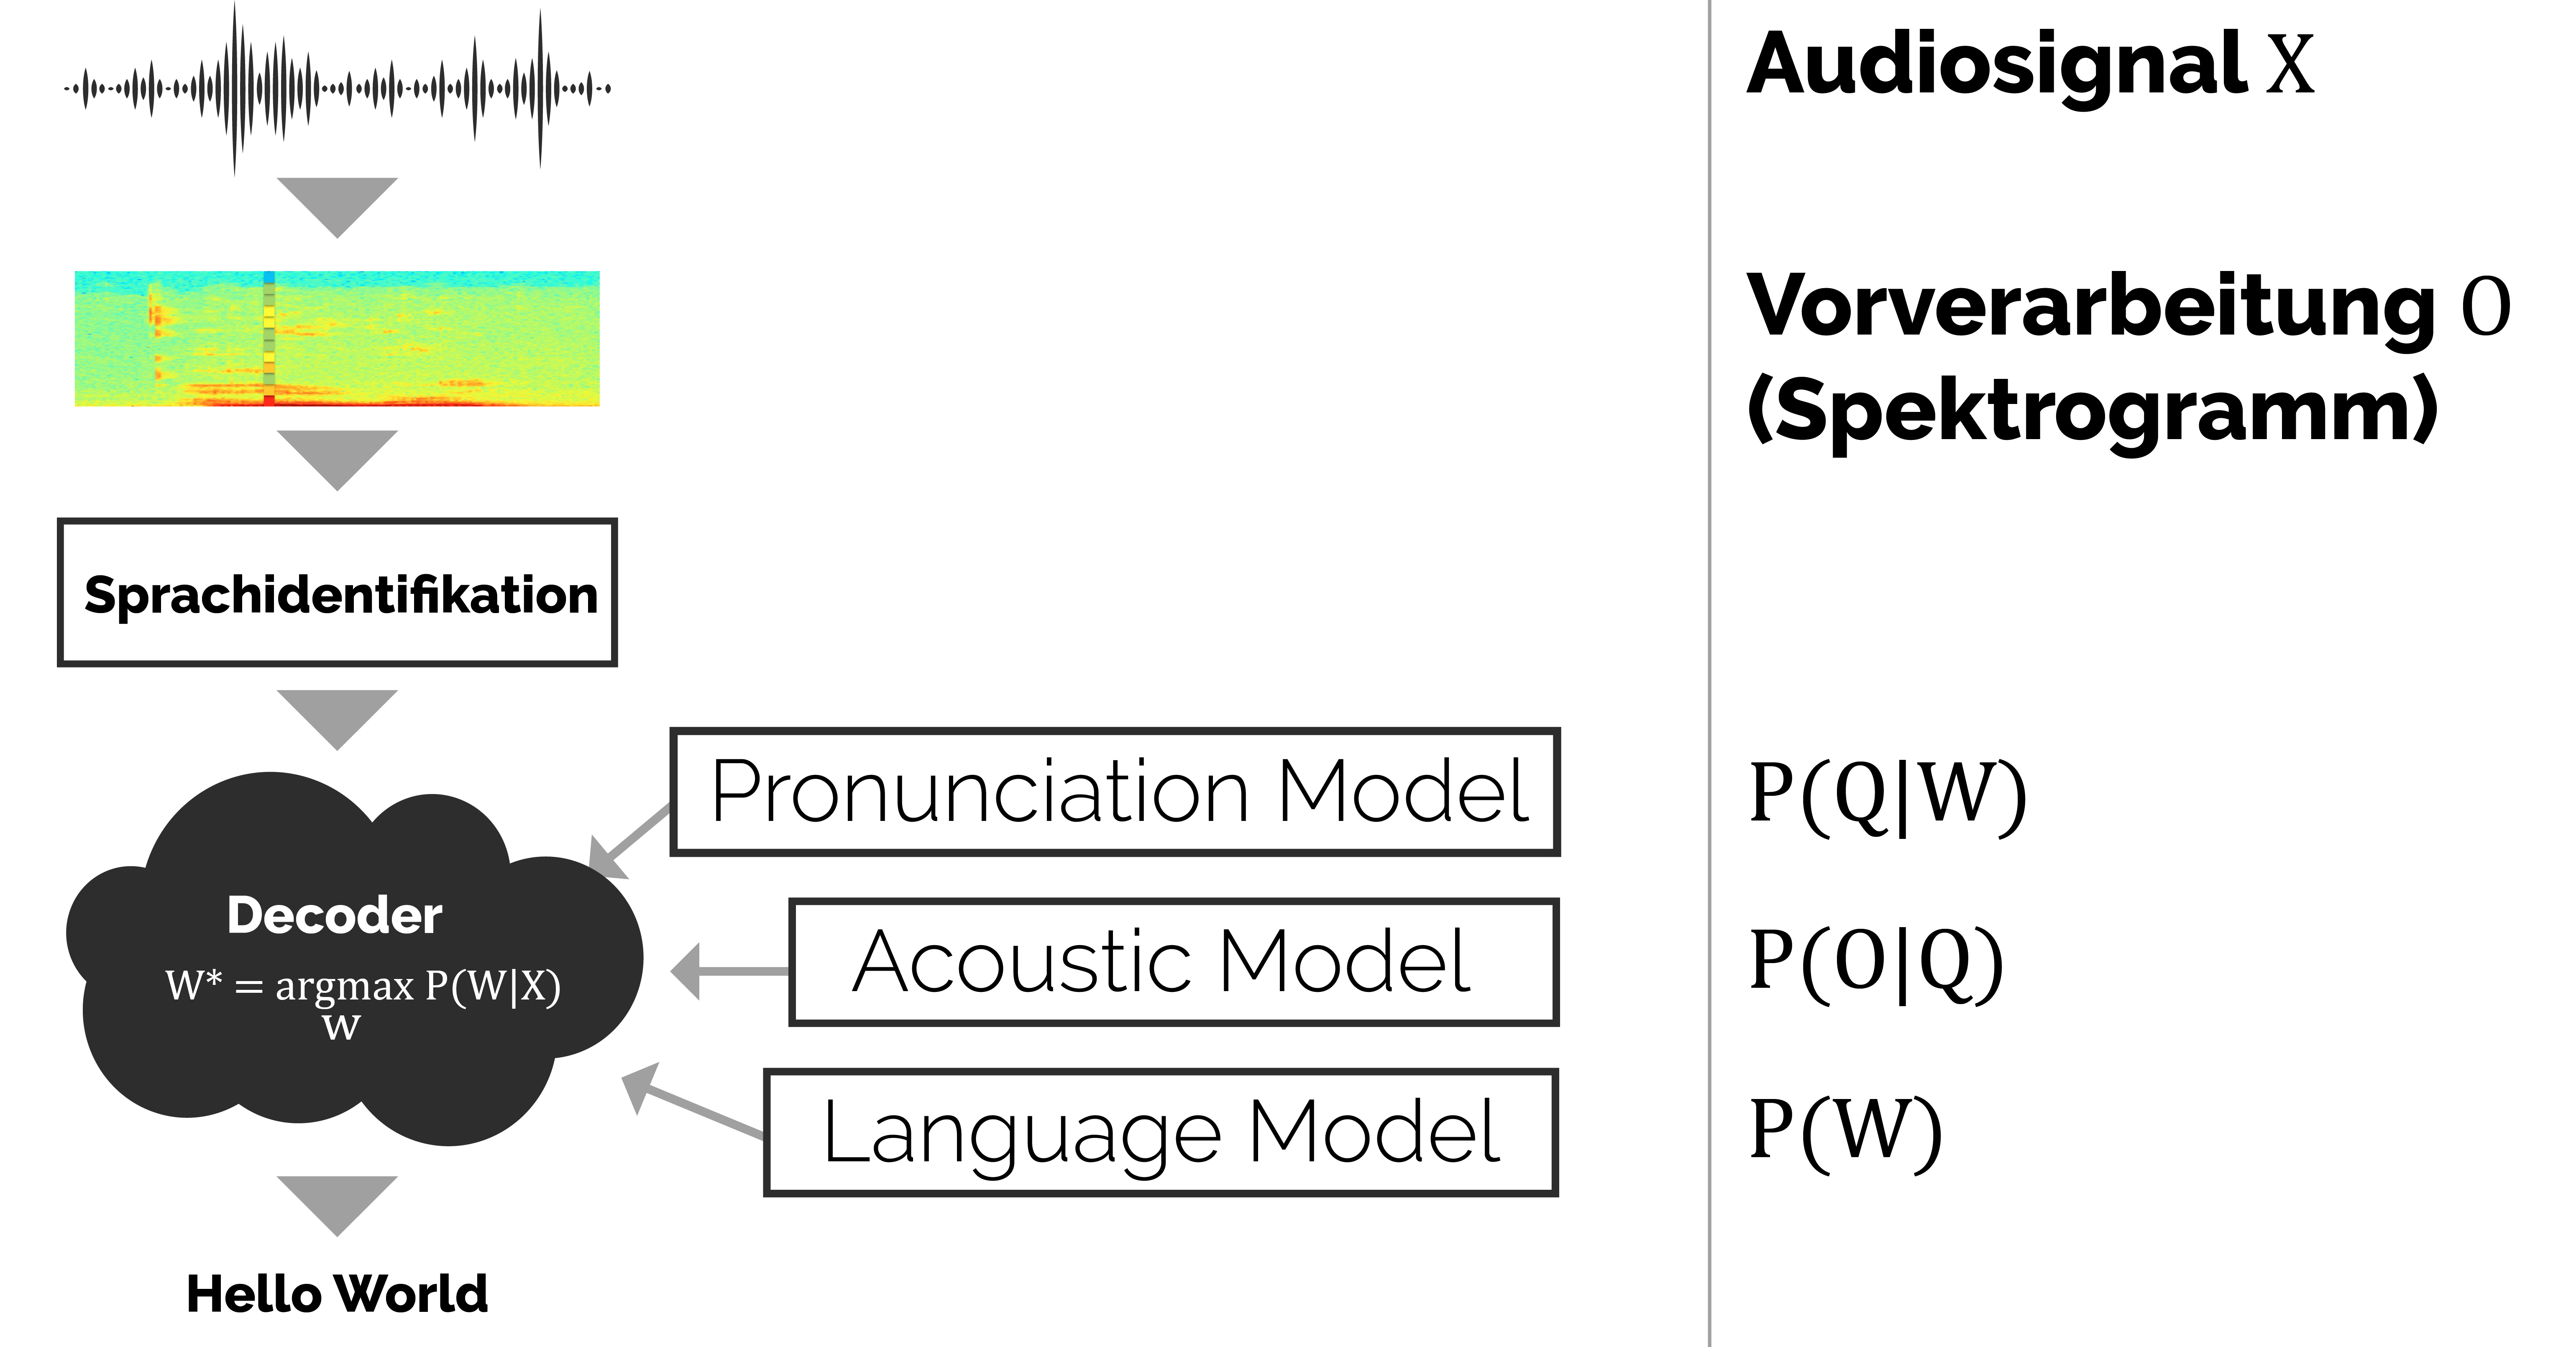
\includegraphics[width=1\linewidth]{images/Presentation-01-01}
    \caption{Pipeline eines Spracherkennungssystems (Nach: ) }%\cite{??}}
    \label{fig:pipeline}
\end{figure}

[1] Automatic Speech Recognition - A Deep Learning Approach https://www.springer.com/de/book/9781447157786
[2] Simons, Gary F. and Charles D. Fennig (eds.). 2018. Ethnologue: Languages of the World, Twenty-first edition. Dallas, Texas: SIL International. Online version: http://www.ethnologue.com
[3] ???
%Die Arbeit lehnt sich dabei an die von Lars Röwekamp verfassten Artikel auf diversen Plattformen an. Durch seine Beiträge manifestierte er seine grenzenlose Inkompetenz. Scheiß auf dich und dein Copyright.
